\documentclass{article}
\usepackage[english, greek]{babel}
\usepackage[LGR, T1]{fontenc}
\usepackage{graphicx}
\usepackage{lipsum}
\usepackage{hyperref}
\hypersetup{
colorlinks=true,
linkcolor=black,
urlcolor=blue}

\begin{document}

    \fontsize{50pt}{35pt}\selectfont
    \centering{\textbf{Αναφορά Εργασίας}}
    \vfill
    \fontsize{20pt}{20pt}\selectfont
    \textbf{Ιόνιο Πανεπιστήμιο}
    
\includegraphics[width=0.4\textwidth]{photos/Ionian_University_seal.png}
    \vfill
    \fontsize{20pt}{20pt}\selectfont
    \textbf{Μάθημα: \\Τεχνολογία Λογισμικού}
    \vfill
    \fontsize{16pt}{16pt}\selectfont
    \textbf{Ομάδα: \\
    - Νικόλαος Τρυπάκης \selectlanguage{english}inf2021229\\
    - \selectlanguage{greek}Στέφανος Σφηναρολάκης \selectlanguage{english}inf2021218\\
    - \selectlanguage{greek}Ορέστης Ραφαήλ Μακρής \selectlanguage{english}inf2021129}

\newpage

\raggedright
\fontsize{15pt}{15pt}\selectfont
\tableofcontents

\newpage \selectlanguage{greek}
\large
\raggedright
\section{Εισαγωγή}
Μας ζητήθηκε η ανάπτυξη μιας \selectlanguage{english}web-based \selectlanguage{greek}εφαρμογής, η οποία παρέχει τις λειτουργίες της φόρτωσης, της ανάλυσης και της οπτικοποίησης δεδομένων μέσω ευέλικτων λειτουργιών. Η εφαρμογή δημιουργήθηκε χρησιμοποιώντας την βιβλιοθήκη \selectlanguage{english}Streamlit,\selectlanguage{greek} ενώ υποστηρίζει διάφορες αναλυτικές και οπτικοποιητικές λειτουργίες.

Στο πλαίσιο αυτό, η εφαρμογή διαθέτει:
\begin{itemize}
    \item Φόρτωση Δεδομένων: Η δυνατότητα φόρτωσης δεδομένων σε μορφή πίνακα από αρχεία δεδομένων.
    \item Οπτικοποίηση Δεδομένων: Οπτικοποιήσεις που επιτρέπουν την εξαγωγή σημαντικών πληροφοριών από τα δεδομένα.
    \item Σύγκριση Αλγορίθμων: Δυνατότητα σύγκρισης της απόδοσης διάφορων αλγορίθμων μηχανικής μάθησης για τα δεδομένα που αναλύονται.
    \item Παρουσίαση: Παρουσίαση των αποτελεσμάτων ανάλυσης.
\end{itemize}
Στόχος είναι η εφαρμογή να αποτελέσει ένα πολύτιμο εργαλείο για την ανάλυση και διευκολία στην ανακάλυψη νέων πληροφοριών από τα δεδομένα των χρηστών.

\newpage

\section{Προγραμματιστικές Επιλογές}
\begin{itemize}
\item \textbf{Θέμα Φιλικό προς τον Χρήστη:} Το αρχείο \selectlanguage{english}app.py\selectlanguage{greek} είναι εφαρμοσμένο για τον χρήστη χρησιμοποιώντας τις δυνατότητες του \selectlanguage{english}Streamlit\selectlanguage{greek} καθώς και της χρήσης του \selectlanguage{english}Streamlit Navigation Bar.\selectlanguage{greek} Αυτές οι επιλογές βελτιώνουν την εμπειρία του χρήστη παρέχοντας ένα οπτικά κατανοητό περιβάλλον ως προς την διάταξη της σελίδας.

\item \textbf{Δομή Κώδικα σε Ανεξάρτητα Μέρη:} Ο κώδικας οργανώνεται σε ξεχωριστά \selectlanguage{english}modules (data\_loader.py, visualization.py, machinelearning.py,    info.py).\selectlanguage{greek} Αυτό επιτρέπει ευκολότερη πλοήγηση, εντοπισμό σφαλμάτων και μελλοντικές ενημερώσεις, καθώς κάθε \selectlanguage{english}module \selectlanguage{greek}επικεντρώνεται σε ένα συγκεκριμένο κομμάτι της λειτουργικότητας της εφαρμογής.

\item \textbf{Λειτουργεία Ανεβάσματος Αρχείων:} Η λειτουργία \selectlanguage{english}st.file\_uploader\selectlanguage{greek} από το \selectlanguage{english}Streamlit\selectlanguage{greek} χρησιμοποιείται για να επιτρέψει στους χρήστες να ανεβάζουν τα αρχεία δεδομένων τους \selectlanguage{english}(CSV, Excel).\selectlanguage{greek} Αυτή η επιλογή παρέχει ευελιξία και άνεση στους χρήστες, επιτρέποντάς τους να αναλύουν τα δικά τους \selectlanguage{english}datasets\selectlanguage{greek} εντός της εφαρμογής.

\item \textbf{Οπτικοποίηση:} Διαδραστικά γραφήματα δημιουργούνται χρησιμοποιώντας το \selectlanguage{english}plotly.express \selectlanguage{greek}στο\selectlanguage{english} module visualization.py. \selectlanguage{greek}Το \selectlanguage{english}Plotly Express\selectlanguage{greek} προσφέρει μια υψηλού επιπέδου διεπαφή για τη δημιουργία εκφραστικών και διαδραστικών οπτικοποιήσεων με ελάχιστο κώδικα. Αυτή η επιλογή βελτιώνει την ανάλυση των δεδομένων επιτρέποντας στους χρήστες να δουν εύκολα τις σχέσεις στα δεδομένα τους.

\item \textbf{Αλγόριθμοι Μηχανικής Μάθησης:} Αλγόριθμοι ταξινόμησης και ομαδοποίησης όπως οι \selectlanguage{english}K-Nearest Neighbors, Support Vector Machine, K-Means \selectlanguage{greek}και \selectlanguage{english}Gaussian Mixture Models\selectlanguage{greek} χρησιμοποιήθηκαν μέσω της βιβλιοθήκης \selectlanguage{english}scikit-learn.\selectlanguage{greek}
\end{itemize}
\newpage

\section{\selectlanguage{english}UML\selectlanguage{greek} Διάγραμμα}

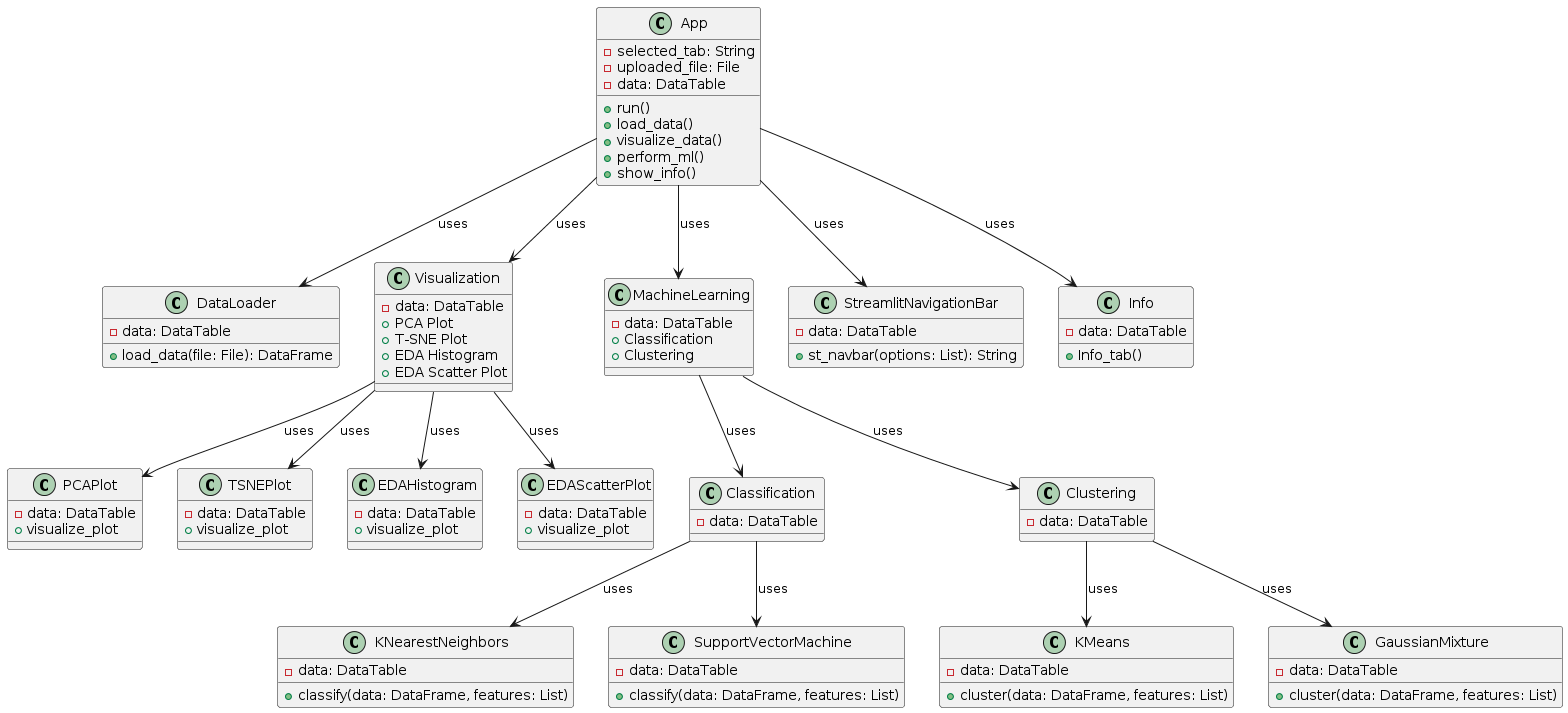
\includegraphics[width=1.25\textwidth]{photos/uml_datagram.png}

\subsection{Κλάσεις Φόρτωσης Δεδομένων}

\textbf{\selectlanguage{english}DataLoader:} \selectlanguage{greek}Αυτή η κλάση είναι υπεύθυνη για τη φόρτωση δεδομένων από αρχεία \selectlanguage{english}CSV \selectlanguage{greek}και \selectlanguage{english}Excel.\selectlanguage{greek} Τα δεδομένα φορτώνονται στο \selectlanguage{english}DataTable.\selectlanguage{greek}

\textbf{\selectlanguage{english}DataTable:} Η κλάση \selectlanguage{english}DataTable \selectlanguage{greek}διαχειρίζεται τα δεδομένα που φορτώθηκαν.

\subsection{Οπτικοποίηση \selectlanguage{english}2D}

Αυτή η κλάση δημιουργεί τα ακόλουθα γραφήματα οπτικοποίησης:

\begin{itemize}
  \item \textbf{\selectlanguage{english}EDAHistogram:} Προβάλλει ιστόγραμμα.
  \item \textbf{\selectlanguage{english}EDAScatterPlot:} Απεικονίζει την κατανομή των δεδομένων χρησιμοποιώντας \selectlanguage{english}scatter plot.\selectlanguage{greek}
  \item \textbf{\selectlanguage{english}PCAPlot:} Παρουσιάζει τα αποτελέσματα της \selectlanguage{english}PCA. \selectlanguage{greek}
  \item \textbf{\selectlanguage{english}TSNEPlot:} Εμφανίζει τα αποτελέσματα του \selectlanguage{english}t-SNE.\selectlanguage{greek}
\end{itemize}

\subsection{Μηχανική Μάθηση}

Αυτή η κλάση περιλαμβάνει λειτουργίες μηχανικής μάθησης. Περιέχει δύο υποσυστήματα:

\begin{itemize}
  \item \textbf{\selectlanguage{english}Classification:} \selectlanguage{greek}Χρησιμοποιείται για την εκτέλεση αλγορίθμων ταξινόμησης.
  \begin{itemize}
    \item \textbf{\selectlanguage{english}KNearestNeighbros}
    \item \textbf{\selectlanguage{english}Support Vector Machine}
  \end{itemize}
  \item \textbf{\selectlanguage{english}Clustering:} \selectlanguage{greek}Χρησιμοποιείται για την εκτέλεση αλγορίθμων ομαδοποίησης.
  \begin{itemize}
    \item \textbf{\selectlanguage{english}KMeans}
    \item \textbf{\selectlanguage{english}GaussianMixture}
  \end{itemize}
\end{itemize}

\subsection{\selectlanguage{english}Tab \selectlanguage{greek}Πληροφοριών}

Η καρτέλα \selectlanguage{english}InfoTab \selectlanguage{greek}παρέχει πληροφορίες σχετικά με την εφαρμογή και τα μέλη της ομάδας που δούλεψαν στην ανάπτυξη της.

\newpage

\section{Εκτέλεσης της Εφαρμογής με \selectlanguage{english}Docker}
Αρχικά, χρειάζεται να κατέβει το \selectlanguage{english}Docker Desktop \selectlanguage{greek}στο σύστημα.

Μετά χρειάζεται η δημιουργία του \selectlanguage{english}dockerfile:
\vspace{0.3 cm}

\textbf{FROM python:3.11.9\\
WORKDIR /app\\
COPY requirements.txt requirements.txt\\
RUN pip install -r requirements.txt\\
COPY . .\\
CMD ["streamlit", "run", "app/app.py"]}\\
\vspace{0.3 cm}
\selectlanguage{greek}Μέσω αυτών των εντολών όπου αποτελούν το περιεχόμενο του αρχείου \selectlanguage{english}"Dockerfile" \selectlanguage{greek}ορίζεται τον ευρετήριο της εφαρμογής, κατεβαίνουν οι απαραίτητες βιβλιοθήκες και μέσω του \selectlanguage{english}Streamlit \selectlanguage{greek}τρέχει το βασικό αρχείο της εφαρμογής.\\

Έπειτα την δημιουργία του αρχείου θα χρειαστεί να εκτελεστούν οι ακόλουθες εντολές:\\
\begin{itemize}
    \item \textbf{\selectlanguage{english}docker build -t "your\_app\_name" .}
    \item \textbf{\selectlanguage{english}docker run -p 8501:8501 "your\_app\_name"}
\end{itemize}

\newpage

\section{\selectlanguage{english}Guide \selectlanguage{greek}της Εφαρμογής}
Κατά την χρήση της εφαρμογής θα πρέπει να χρησιμοποιηθεί ένα αρχείο με \selectlanguage{english}data \selectlanguage{greek}από τον χρήστη. Για το παράδειγμα του \selectlanguage{english}guide\selectlanguage{greek} θα χρησιμοποιηθεί ένα αρχέιο με \selectlanguage{english}data\selectlanguage{greek} από δείγματα λουλουδιών ίρις.\\\vspace{0.3 cm}

\subsection{Είσοδος στην εφαρμογή}

Κατά την είσοδο στην ιστοσελίδα ο χρήστης θα βρεθεί με την επιλογή να εισάγει τα δεδομένα του μέσω της επιλογής σχετικού αρχείου.\\\vspace{0.3 cm}
\begin{figure}[h!]
  \centering
  
\includegraphics[width=0.6\textheight]{photos/upload_button.png}
  \caption{\selectlanguage{english}Data Uploader Button}
  \label{fig:DataLoader}
\end{figure}

\newpage

\subsection{\selectlanguage{english}Data Loader Tab}
Μετά την εισαγωγή του αρχείου δεδομένων, είναι αρκετά εμφανής η ύπαρξη διαφορετικών σελιδών όπου ο χρήστης έχει διάφορες δυνατότητες σε κάθε μία ξεχωριστά.\\
\vspace{0.3 cm}
Η πρώτη σελίδα της εφαρμογής είναι αυτή του \selectlanguage{english}Data Loader \selectlanguage{greek} όπου ο χρήστης μπορεί να δει τα δεδομένα του καθώς και τις ετικέτες τους πατώντας το κουμπί \textbf{\selectlanguage{english}Show Data}.

\begin{figure}[h!]
  \centering
  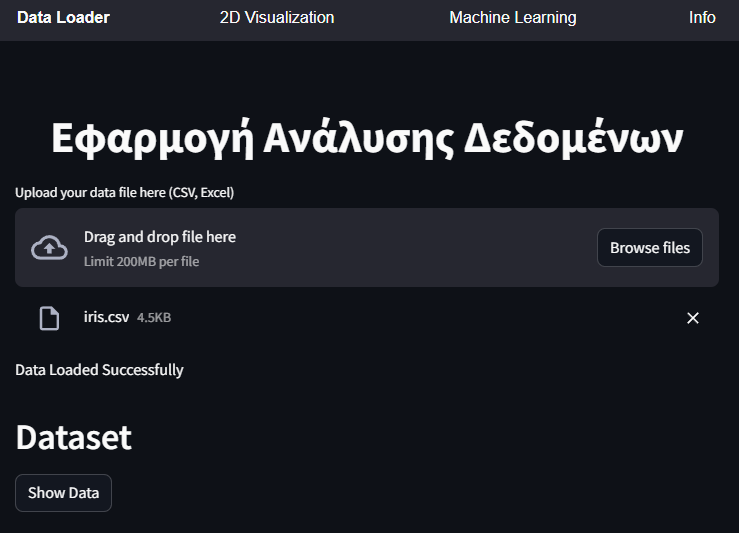
\includegraphics[width=0.6\textheight]{photos/data_loader.png}
  \caption{\selectlanguage{english}Data Loader}
  \label{fig:DataLoader}
\end{figure}
\newpage
Παράδειγμα φορτωμένων δεδομένων:
\begin{figure}[h!]
  \centering
  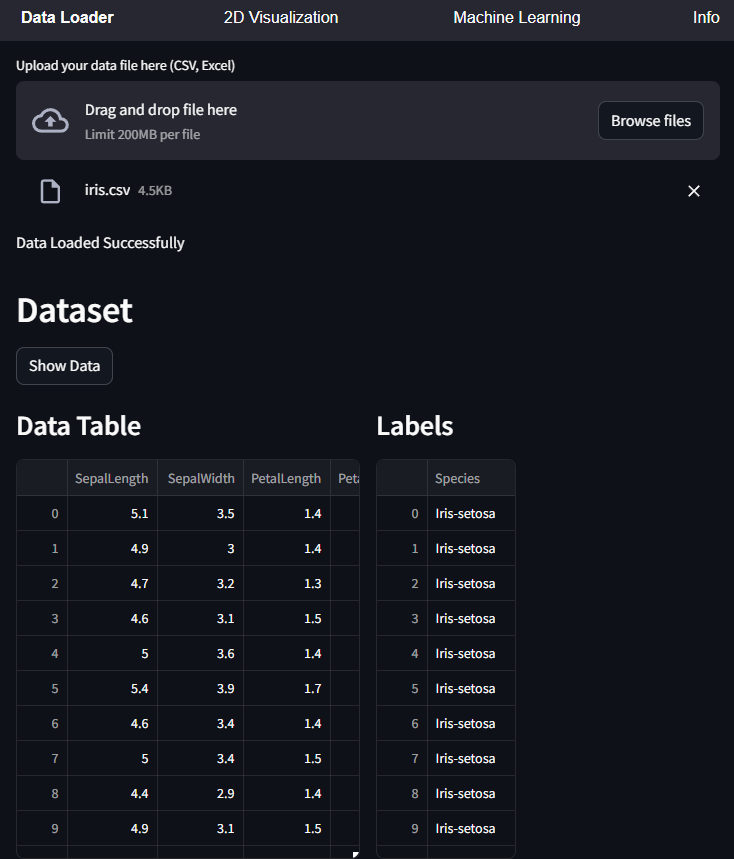
\includegraphics[width=0.6\textheight]{photos/loaded_data.png}
  \caption{Φορτωμένα Δεδομένα}
  \label{fig:Loaded Data}
\end{figure}

\newpage
\subsection{\selectlanguage{english}2D Visualization}
Στην δεύτερη σελίδα \selectlanguage{english}"2D Visualization" \selectlanguage{greek}ο χρήστης έχει την δυνατότητα να εκτελέσει οπτικοποιήσεις έτοιμων αλγορίθμων \selectlanguage{english}(PCA, t-SNE) \selectlanguage{greek}με τα δεδομένα του και να τα αναλύσει με κατάλληλα σχήματα \selectlanguage{english}(EDA Charts)\selectlanguage{greek} μέσω επίλογης από το διαθέσιμο μενού.
\begin{figure}[h!]
  \centering
  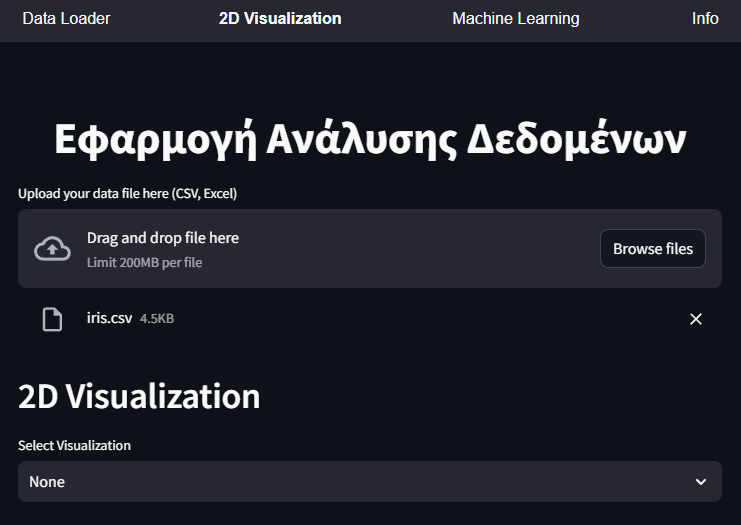
\includegraphics[width=0.6\textheight]{photos/2d_tab.png}
  \caption{\selectlanguage{english}2D Visualization}
  \label{fig:2DVisualization}
\end{figure}
\newpage
\subsubsection{\selectlanguage{english}PCA Plot}
\begin{figure}[h!]
  \centering
  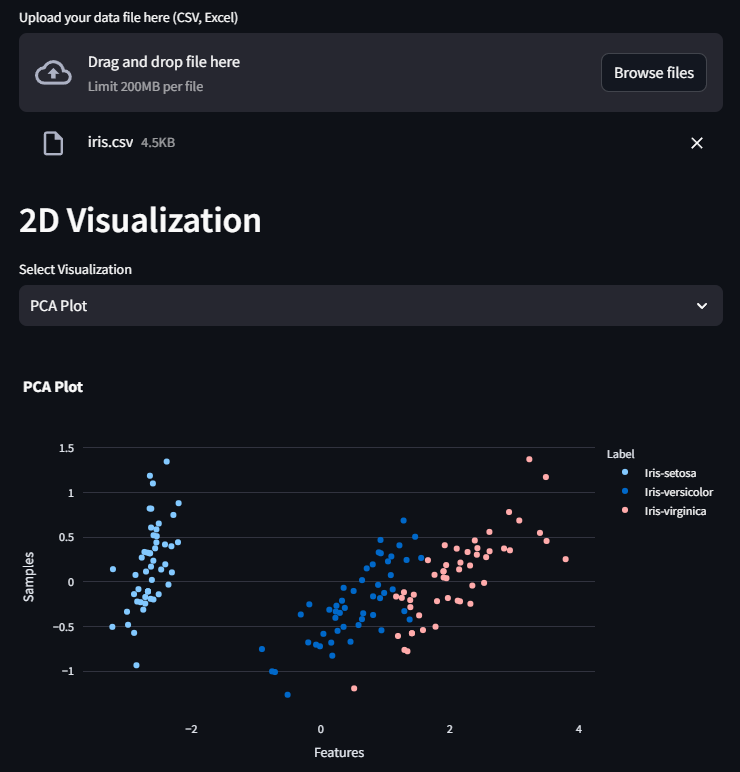
\includegraphics[width=0.6\textheight]{photos/pca.png}
  \caption{\selectlanguage{english}PCA Plot}
  \label{fig:PCA Plot}
\end{figure}
\vspace{0.3 cm}
Το \selectlanguage{english}PCA \selectlanguage{greek}μετασχηματίζει τα δεδομένα από τον αρχικό χώρο των 4 διαστάσεων (μήκος και πλάτος πετάλων και σέπαλων) σε ένα \selectlanguage{english}2D \selectlanguage{greek}διάγραμμα που διατηρεί τη μέγιστη δυνατή διακύμανση. Οι τρεις κατηγορίες \selectlanguage{english}(Iris-setosa, Iris-versicolor, Iris-virginica) \selectlanguage{greek}απεικονίζονται σε διαφορετικά χρώματα, επιτρέποντας τον οπτικό διαχωρισμό τους.
\newpage
\subsubsection{\selectlanguage{english}t-SNE Plot}
\begin{figure}[h!]
  \centering
  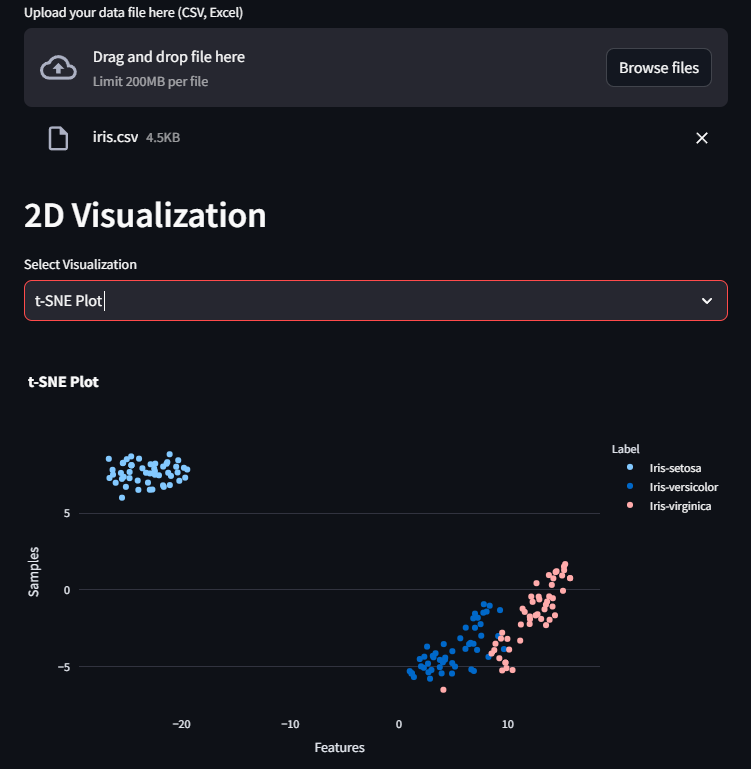
\includegraphics[width=0.6\textheight]{photos/t-sne.png}
  \caption{\selectlanguage{english}t-SNE Plot}
  \label{fig:TSNE Plot}
\end{figure}

\vspace{0.3 cm}
Το {\selectlanguage{english}t-SNE {\selectlanguage{greek}χαρτογραφεί τα δεδομένα σε έναν {\selectlanguage{english}2D {\selectlanguage{greek}χώρο, διατηρώντας τις τοπικές σχέσεις μεταξύ των σημείων. Αυτό το καθιστά εξαιρετικά χρήσιμο για την οπτικοποίηση συστάδων στα δεδομένα {\selectlanguage{english}Iris,{\selectlanguage{greek} δείχνοντας πώς τα σημεία δεδομένων συγκεντρώνονται και διαχωρίζονται μεταξύ των τριών κατηγοριών. Όπως και πριν, οι τρεις κατηγορίες απεικονίζονται σε διαφορετικά χρώματα.
\newpage

\subsubsection{\selectlanguage{english}EDA \selectlanguage{greek}Διαγράμματα}
\vspace{0.3 cm}
\textbf{Ιστόγραμμα}
\begin{figure}[h!]
  \centering
  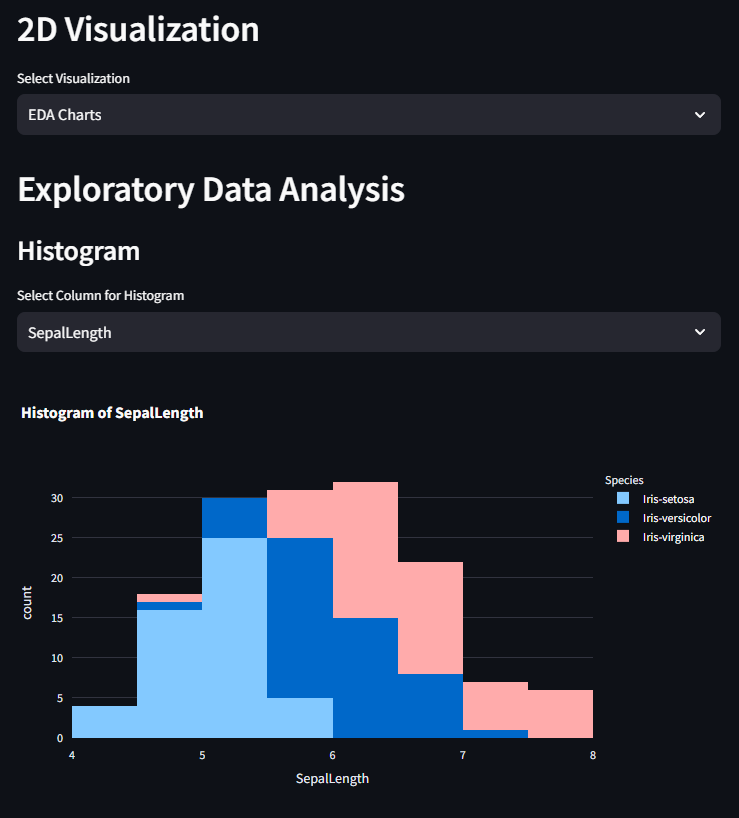
\includegraphics[width=0.6\textheight]{photos/histogram.png}
  \caption{Ιστόγραμμα}
  \label{fig:Histogram}
\end{figure}
\\ \vspace{0.3 cm}
Επιλέγοντας μια στήλη από τα δεδομένα \selectlanguage{english}Iris \selectlanguage{greek}(π.χ. μήκος σεπάλου), το ιστόγραμμα δείχνει πόσο συχνά εμφανίζονται συγκεκριμένες τιμές για αυτή τη μεταβλητή. Τα δεδομένα χρωματίζονται ανάλογα με την κατηγορία τους, επιτρέποντας την ανάλυση της κατανομής κάθε κατηγορίας.
\newpage

\textbf{Διάγραμμα Διασποράς}
\begin{figure}[h!]
  \centering
  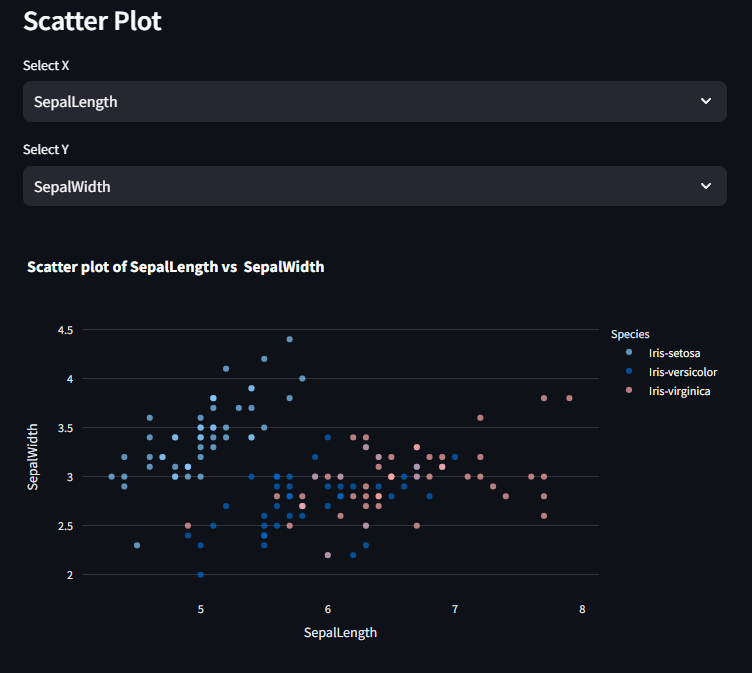
\includegraphics[width=0.6\textheight]{photos/scatter_plot.png}
  \caption{Διάγραμμα Διασποράς}
  \label{fig:ScatterPlot}
\end{figure}
\\ \vspace{0.3 cm}
Επιλέγοντας δύο στήλες από τα δεδομένα \selectlanguage{english}Iris\selectlanguage{greek} (π.χ. μήκος σεπάλου και πλάτος σεπάλου), το διάγραμμα διασποράς δείχνει πώς οι τιμές αυτών των μεταβλητών σχετίζονται μεταξύ τους. Τα δεδομένα χρωματίζονται σύμφωνα με τις κατηγορίες τους
\newpage
\subsection{Μηχανική Μάθηση}
Στην τρίτη σελίδα \selectlanguage{english}"Machine Learning" \selectlanguage{greek}ο χρήστης μπορεί να χρησιμοποιήσει αλγορίθμους μηχανικής μάθησης έχοντας δύο επιλογές: Αλγορίθμους Κατηγοριοποίησης ή  Αλγορίθμους Ομαδοποίησης. Αυτοί οι αλγόριθμοι βγάζουν ποσοστό επιτυχίας και γίνεται σύγκριση μεταξύ τους έτσι ώστε ο χρήστης να γνωρίσει ποιος είναι πιο συμβατός με τα δεδομένα του.
\begin{figure}[h!]
  \centering
  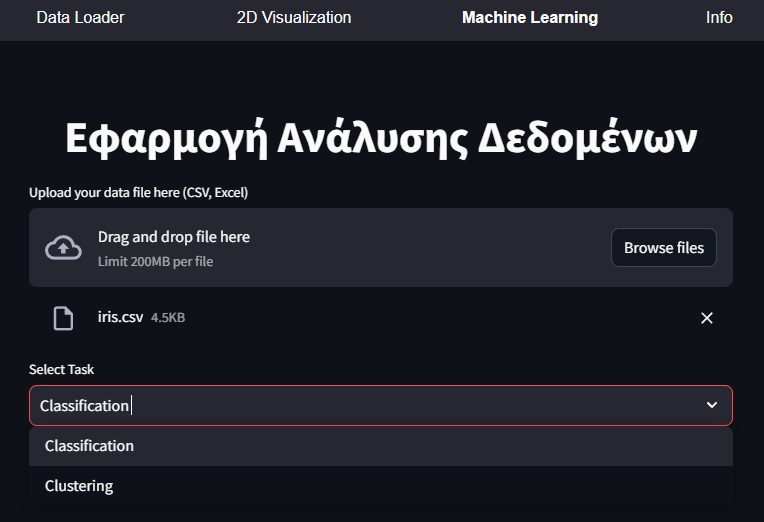
\includegraphics[width=0.6\textheight]{photos/machine_learning.png}
  \caption{\selectlanguage{english}Machine Learning}
  \label{fig:MachineLearning}
\end{figure}

\newpage
\textbf{Παράδειγμα Κατηγοριοποίησης}
\begin{figure}[h!]
  \centering
  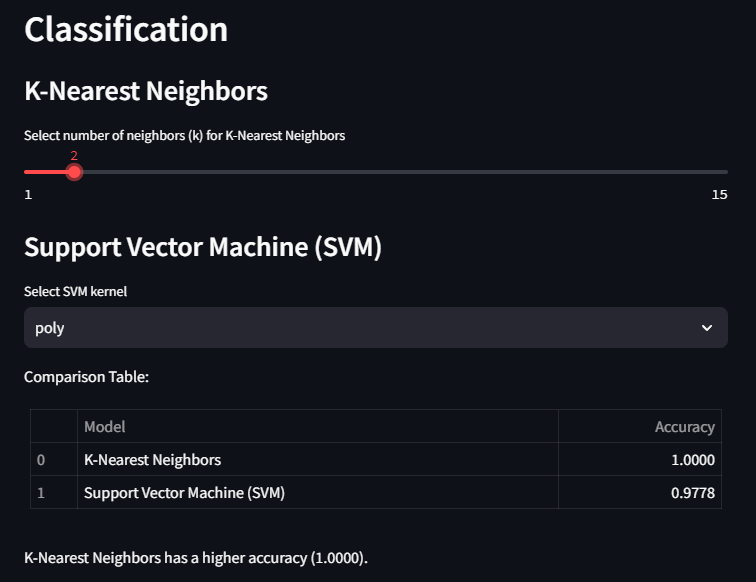
\includegraphics[width=0.6\textheight]{photos/classification.png}
  \caption{\selectlanguage{english}Classification}
  \label{fig:Classification}
\end{figure} \\
\textbf{\selectlanguage{english}KNN VS SVM:} \selectlanguage{greek}Το \selectlanguage{english}KNN \selectlanguage{greek}επιτυγχάνει υψηλότερη ακρίβεια (1.0) λόγω της απλότητας και του καθαρού διαχωρισμού στο σύνολο δεδομένων \selectlanguage{english}Iris. \selectlanguage{greek}Το \selectlanguage{english}SVM \selectlanguage{greek}με πολυωνυμικό πυρήνα (0.97) είναι ελαφρώς λιγότερο ακριβές λόγω της πολυπλοκότητας του.

\newpage
\textbf{Παράδειγμα Ομαδοποίησης}
\begin{figure}[h!]
  \centering
  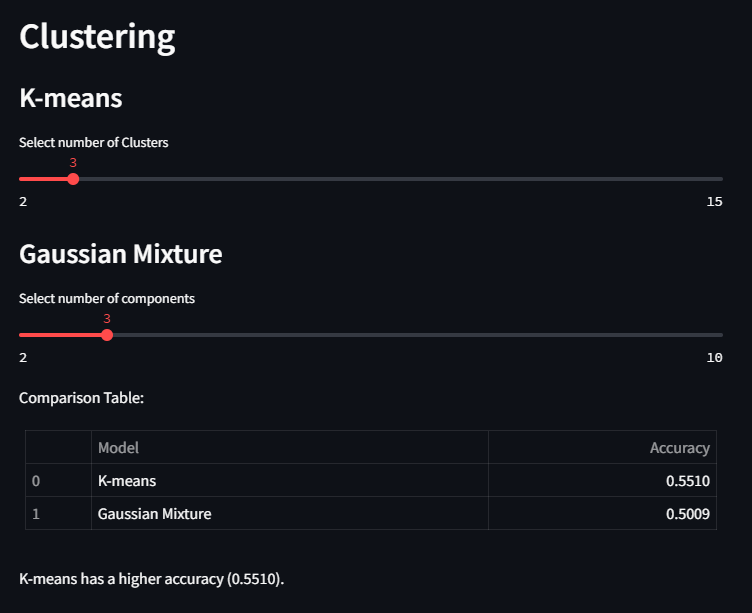
\includegraphics[width=0.6\textheight]{photos/clustering.png}
  \caption{\selectlanguage{english}Clustering}
  \label{fig:Clustering}
\end{figure} \\
\textbf{\selectlanguage{english}K-means VS GM:} \selectlanguage{greek}Το \selectlanguage{english}K-means\selectlanguage{greek} αποδίδει λίγο καλύτερα (0.55) λόγω της προσέγγισής του με κεντροειδή, ενώ το \selectlanguage{english}Gaussian Mixture (0.50)\selectlanguage{greek} δυσκολεύεται με τη φύση των δεδομένων αν αυτά δεν ακολουθούν κανονική κατανομή.

\newpage
\section{Κύκλος Ζωής Έκδοσης Λογισμικού}
Για την ανάπτυξη της \selectlanguage{english}web-based\selectlanguage{greek} εφαρμογής για εξόρυξη και ανάλυση δεδομένων, θα χρησιμοποιήσουμε το \selectlanguage{english}Agile. \selectlanguage{greek}Αυτό το μοντέλο μας επιτρέπει συνεχείς βελτιώσεις και προσαρμογές μέσω επαναλαμβανόμενων κύκλων ανάπτυξης \selectlanguage{english}(sprints).\selectlanguage{greek}\\ Παρακάτω περιγράφεται το προσαρμοσμένο \selectlanguage{english}Agile\selectlanguage{greek} μοντέλο που θα ακολουθήσουμε:
\begin{itemize}
    \item \textbf{Ανάλυση των Απαιτήσεων}
        \begin{itemize}
            \item Συλλογή και ανάλυση των απαιτήσεων των χρηστών μέσω διάφορων τρόπων συλλογής \selectlanguage{english}feedback.
            \item \selectlanguage{greek}Καθορισμός των βασικών λειτουργιών και χαρακτηριστικών της εφαρμογής.
        \end{itemize}
    \item \textbf{Ανάπτυξη Λειτουργιών}
        \begin{itemize}
            \item Σχεδιασμός των \selectlanguage{english}tasks\selectlanguage{greek} και των στόχων για κάθε χρονικό όριο που έχει τεθεί (\selectlanguage{english}sprint).\selectlanguage{greek}
            \item Παρακολούθηση της προόδου και επίλυση των προβλημάτων.
        \end{itemize}
    \item \textbf{\selectlanguage{english}Testing \selectlanguage{greek}και Υποστήριξη}
        \begin{itemize}
            \item Δοκιμές από τους χρήστες για την εξασφάλιση της ικανοποίησης των απαιτήσεων.
            \item Δοκιμή λογισμικού για την εξασφάλιση της ορθότητας του κώδικα.
            \item Παροχή υποστήριξης και εκπαίδευσης προς στους χρήστες.
        \end{itemize}
\end{itemize}
\vspace{0.3 cm}
Για να διατεθεί η εφαρμογή σε ευρύ κοινό, θα εξασφαλίσουμε την ευχρηστία, την αξιοπιστία και την ασφάλεια της εφαρμογής. Θα παρέχουμε τεκμηρίωση και οδηγίες χρήσης, και θα διασφαλίσουμε ότι η εφαρμογή μπορεί να υποστηρίξει πολλούς χρήστες ταυτόχρονα μέσω δοκιμών φορτίου και βελτιστοποίησης απόδοσης.
Με αυτήν την προσέγγιση, η ανάπτυξη της εφαρμογής θα είναι συνεχής και ευέλικτη, επιτρέποντας την προσαρμογή στις ανάγκες των χρηστών και την αντιμετώπιση πιθανών προβλημάτων που μπορεί να προκύψουν κατά τη διάρκεια της ανάπτυξης.

\newpage
\section{Περιγραφή της συνεισφοράς κάθε μέλους της ομάδας}
\vspace{0.3 cm}
\fontsize{14pt}{14pt}\selectfont
\textbf{\selectlanguage{english}Data Loader Tab:}\\
Στην δημιουργία του \selectlanguage{english}Data Loader Tab \selectlanguage{greek}είχε συνεισφορά ο Νικόλαος Τρυπάκης.\\ \vspace{0.3 cm}
\textbf{\selectlanguage{english}2D Visualization Tab:}\\
Στην δημιουργία του \selectlanguage{english}2D Visualization Tab \selectlanguage{greek}είχε συνεισφορά ο Νικόλαος Τρυπάκης.\\ \vspace{0.3 cm}
\textbf{\selectlanguage{english}Machine Learning Tab:}\\
Στην δημιουργία του \selectlanguage{english}Machine Learning Tab \selectlanguage{greek}είχαν συνεισφορά ο Ορέστης Ραφαήλ Μακρής και ο Στέφανος Σφηναρολάκης.\\ \vspace{0.3 cm}
\textbf{\selectlanguage{english}Info Tab:}\\
Στην δημιουργία του \selectlanguage{english}Info Tab \selectlanguage{greek}είχε συνεισφορά ο Στέφανος Σφηναρολάκης.\\ \vspace{0.3 cm}
\textbf{\selectlanguage{english}UML:}\\
Στην δημιουργία του \selectlanguage{english}Info Tab \selectlanguage{greek}είχε συνεισφορά ο Ορέστης Ραφαήλ Μακρής.\\ \vspace{0.3 cm}
\textbf{Μοντέλο Κύκλου Ζωής Λογισμικού \\και \selectlanguage{english}Latex:}\\
Στην δημιουργία του Μοντέλου Κύκλου Ζωής του Λογισμικού και έκθεσης \selectlanguage{english}Latex \selectlanguage{greek}είχε συνεισφορά ο Νικόλαος Τρυπάκης.\\ \vspace{0.3 cm}

\newpage
\section{\selectlanguage{english}Github Repositories}
\textbf{Νικόλαος Τρυπάκης \selectlanguage{english}inf2021229}
\begin{itemize}
    \selectlanguage{english}
    \item Profile: \href{https://github.com/inf2021229}{inf2021229}
    \item Project: \href{https://github.com/inf2021229/sw}{App Repository}
    \item Latex files: \href{https://github.com/inf2021229/latex}{Latex Repository}
    \item UML diagram: \href{https://github.com/inf2021229/uml}{UML Repository}
\end{itemize}
\vspace{0.3 cm}
\textbf{Στέφανος Σφηναρολάκης \selectlanguage{english}inf2021218}
\begin{itemize}
    \selectlanguage{english}
    \item Profile: \href{https://github.com/StefanosSfinarolakis}{inf2021218}
    \item Project: \href{https://github.com/StefanosSfinarolakis/sw}{App Repository}
    \item Latex files: \href{https://github.com/StefanosSfinarolakis/latex}{Latex Repository}
    \item UML diagram: \href{https://github.com/StefanosSfinarolakis/uml}{UML Repository}
\end{itemize}
\vspace{0.3 cm}
\textbf{Ορέστης Ραφαήλ Μακρής \selectlanguage{english}inf2021129}
\begin{itemize}
    \selectlanguage{english}
    \item Profile: \href{https://github.com/inf2021129}{inf2021129}
    \item Project: \href{https://github.com/inf2021129/sw}{App Repository}
    \item Latex files: \href{https://github.com/inf2021129/latex}{Latex Repository}
    \item UML diagram: \href{https://github.com/inf2021129/uml}{UML Repository}
\end{itemize}
\vspace{0.3 cm}
\textbf{Ομάδας}
\begin{itemize}
    \selectlanguage{english}
    \item Profile: \href{https://github.com/TexnologiaLogismikouProject}{Team}
    \item Project: \href{https://github.com/TexnologiaLogismikouProject/sw}{App Repository}
    \item Latex files: \href{https://github.com/TexnologiaLogismikouProject/latex}{Latex Repository}
    \item UML diagram: \href{https://github.com/TexnologiaLogismikouProject/uml}{UML Repository}
\end{itemize}
\end{document}